\chapter{Results}
In this section, the results of the project will be discussed.

\section{System Integration}
This section details the physical system and the integration of the hardware. This includes power consumption, system layout, and component failures or difficulties. The system diagram shown in Figure \ref{masdr_system_diagram} will be explained in detail in this section.
\begin{figure}[!h]
	\centering
	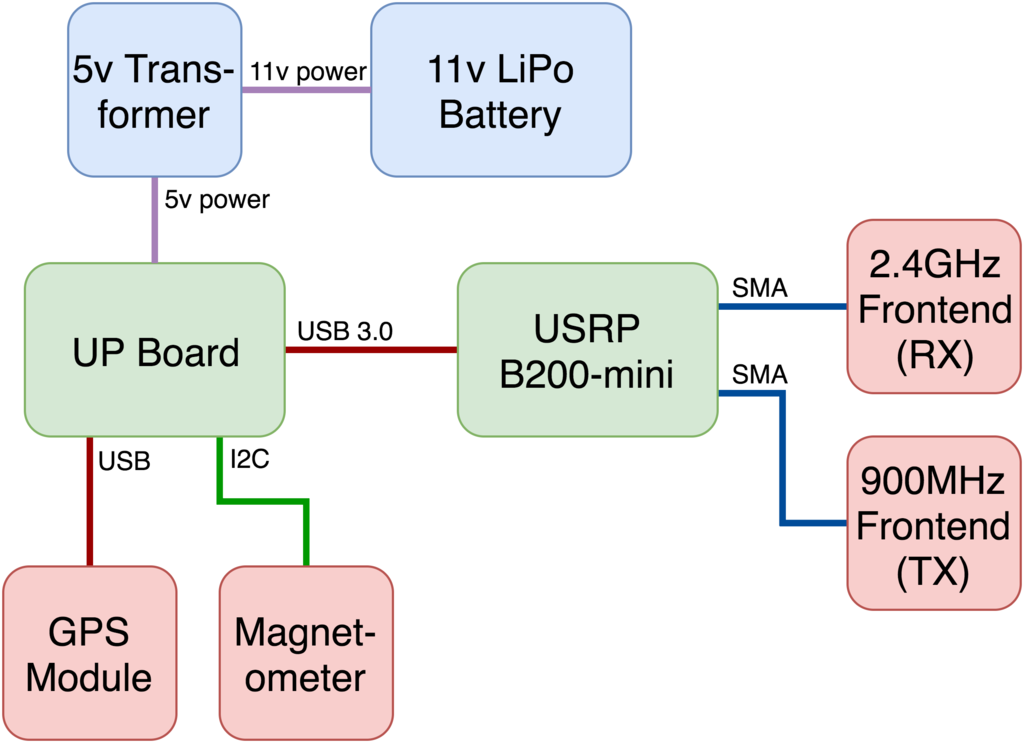
\includegraphics[width=0.70\textwidth]{img/masdr_system_diagram.png}
	\caption{MASDR system diagram detailing the connections between each component.}
	\label{fig:masdr_system_diagram}
\end{figure}\par
The encasing for the system was designed in SOLIDWORKS. It was fabricated using wood panels and a laser cutter. The encasing was designed to be as minimal as possible to reduce the weight of the system. This was done by cutting holes in the panels to remove as much material as possible and using metal supports instead of wooden walls. The metal supports were used in each of the corners to connect the two wooden panels as seen in Figure \ref{fig:connectors}.
\begin{figure}[!h]
	\centering
	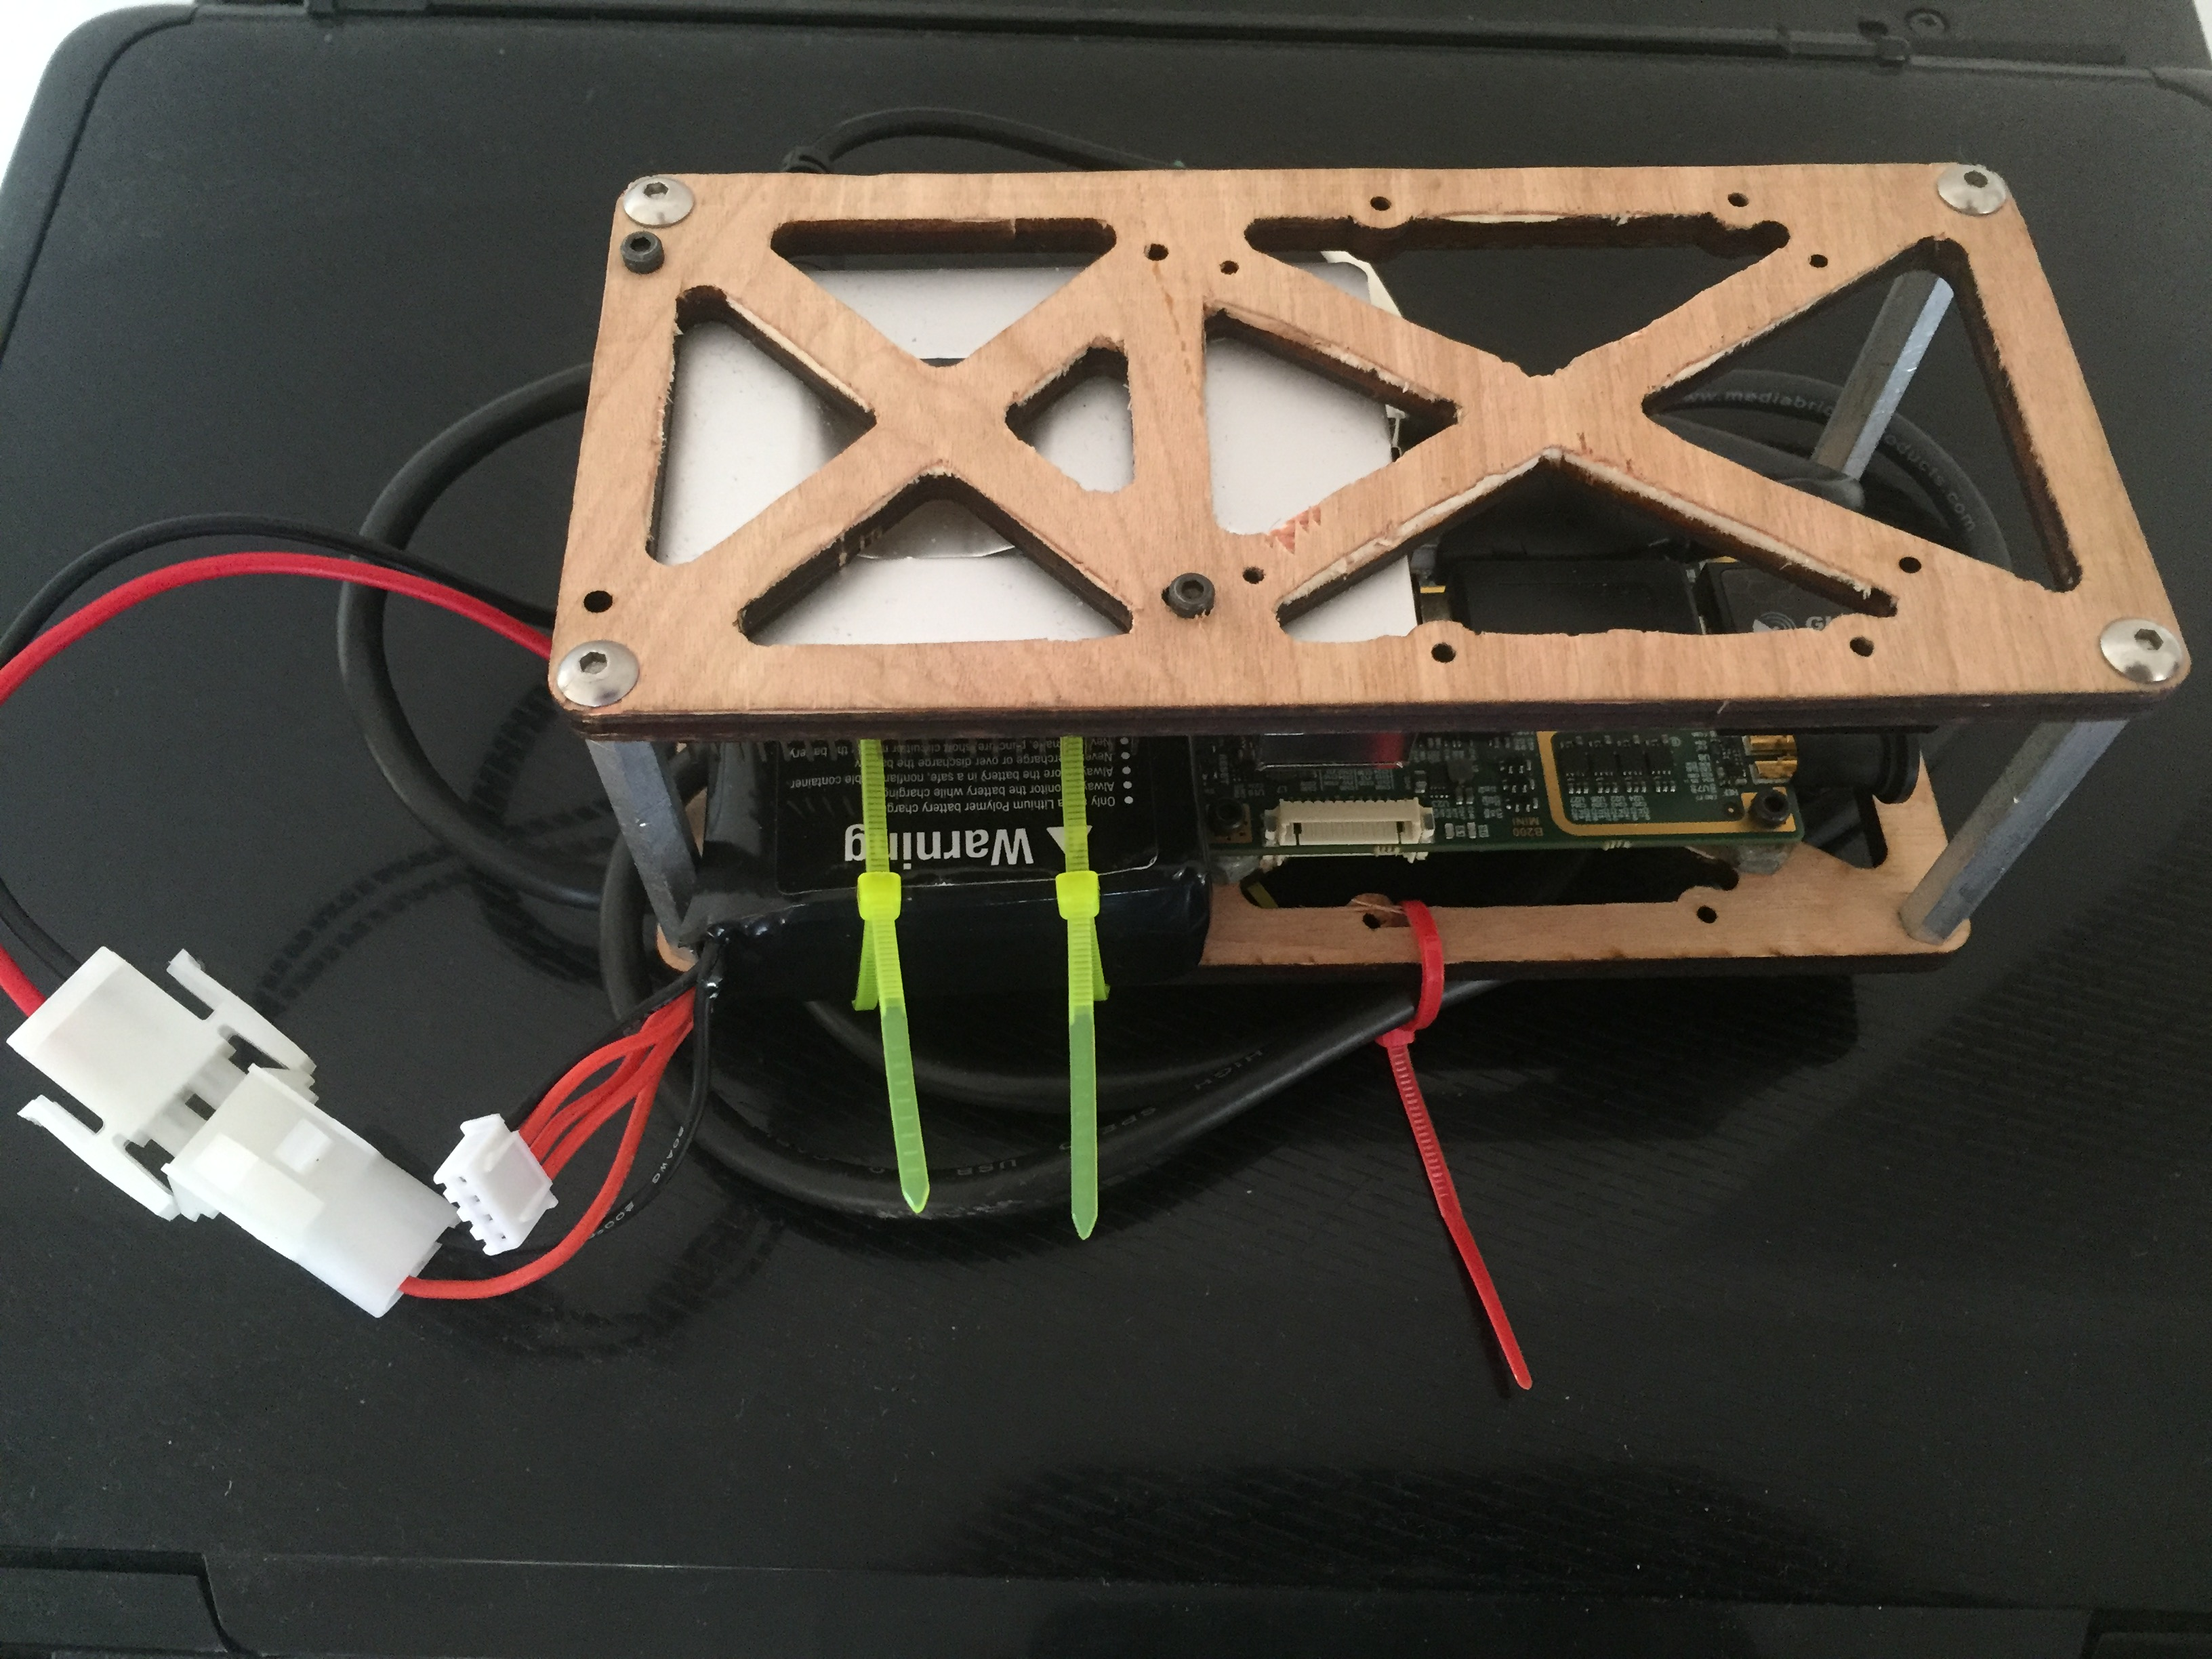
\includegraphics[width=0.70\textwidth]{img/Overhead_of_box.JPG}
	\caption{Overhead view of the encasing of the MASDR system}
	\label{fig:overhead_of_box}
\end{figure}\par
The two wooden panels were created identically to reduce design time and fabrication time. Screw holes were precut into the wood to ensure mounting the components wouldn't split the wood. This enclosure was mounted to the bottom of the drone using the hardware mount on the drone detailed in Section \ref{Mounting}. \par

To power the system, an 11V LiPo battery was used in combination with a 5V transformer to step down the voltage for use by the UP Board. The battery and converter were connected using connectors seen in Figure \ref{fig:connectors}, so that the battery could be disconnected when it is not in use. To prevent any mishandling of plugging the battery in backwards, a male molex connector was soldered to the transformer and a female molex connector was soldered to the battery.
\begin{figure}[!h]
	\centering
	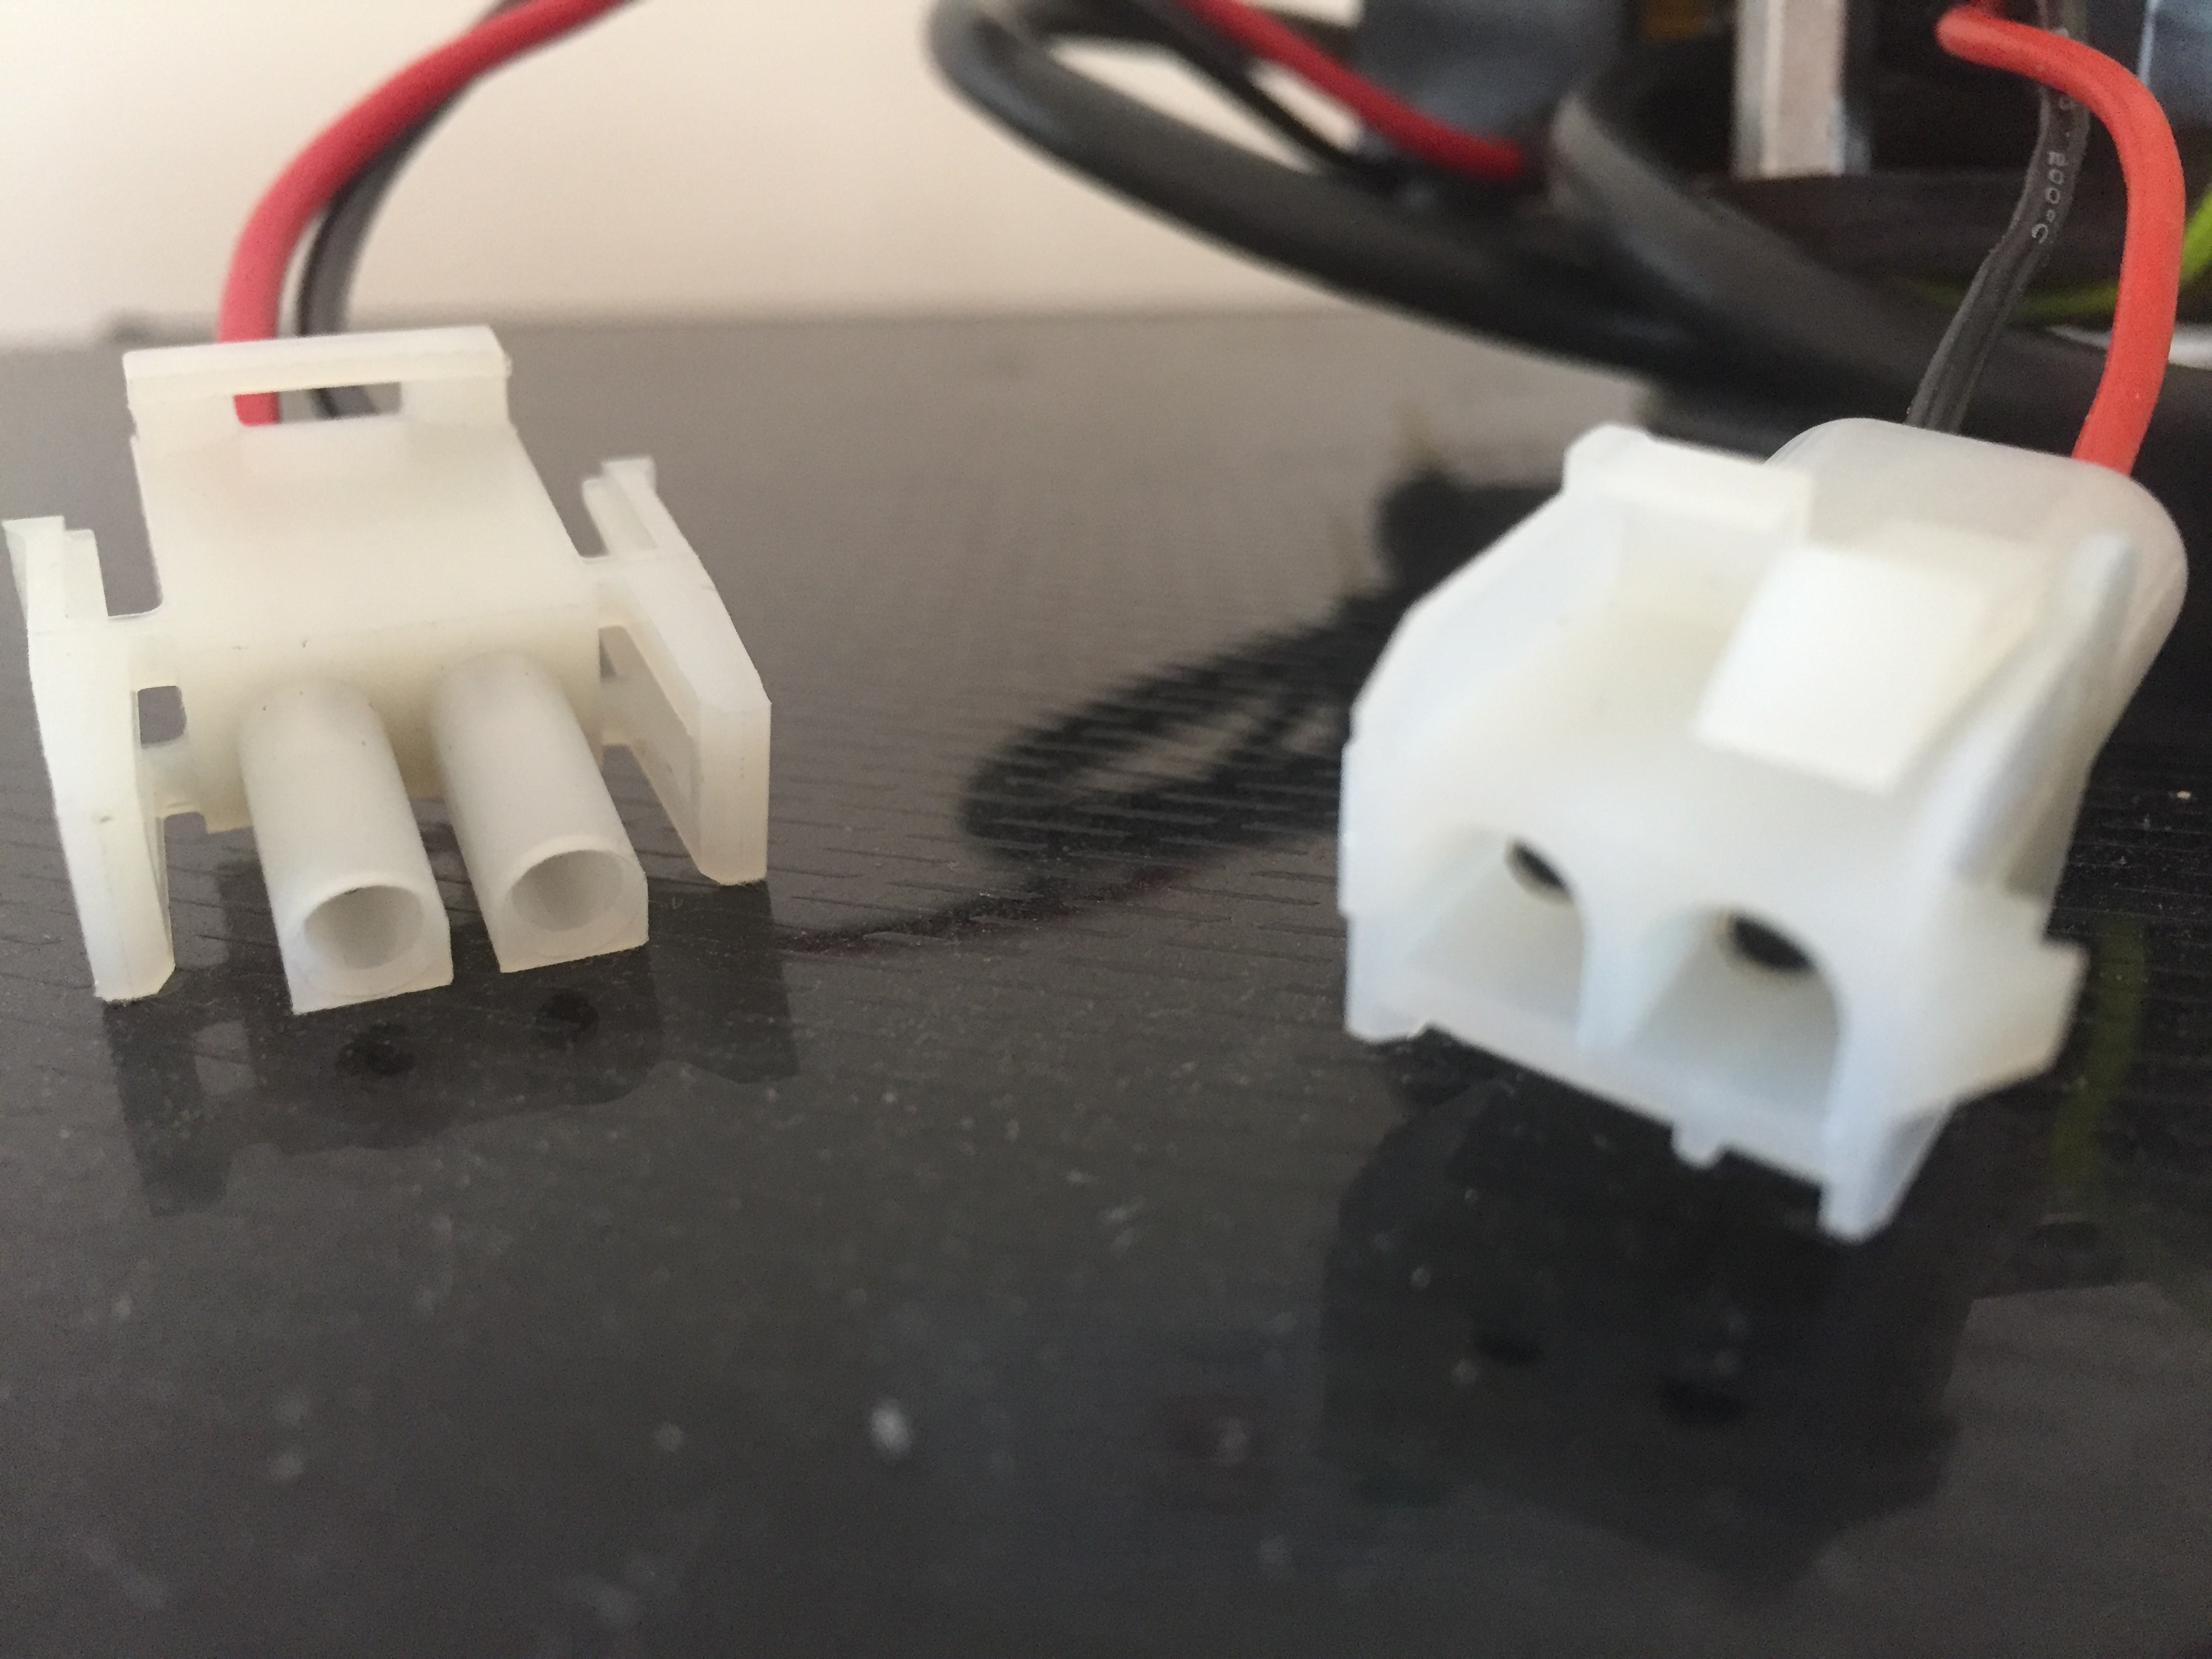
\includegraphics[width=0.70\textwidth]{img/connectors.JPG}
	\caption{Connectors for the battery. The male molex connector (left) is connected to the transformer and the female molex connector (right) is connected to the LiPo battery.}
	\label{fig:connectors}
\end{figure}\par
There were two transformers that were purchased, the Nextrox converter was the one that directly converted 12V down to 5V at 3A, and the DROK converter was the other which was an adjustable knob that ranged from 8V-35V to 1.5V-24V at 5A. Unfortunately the first transformer worked for the first few trails and the second just outright did not work out of the box. The first transformer that was used in the system failed because it became disconnected from the UP Board when power was applied. This transformer was a buck converter which can fail when an output isn't connected due of the failure of a MOSFET or diode. The second transformer's adjustable knob did not change the ratio at which the voltage was being output despite multiple attempts and methods. A new transformer was purchased to replace the malfunctioning transformers. \par

The UP Board is connected to the 5V transformer using a barrel jack. The male connector was soldered onto the output of the transformer. The UP Board is the main system with everything else connected to it through USB or I2C. It was mounted upside down on the top panel as shown in Figure \ref{fig:box_usb_view}.
\begin{figure}[!h]
	\centering
	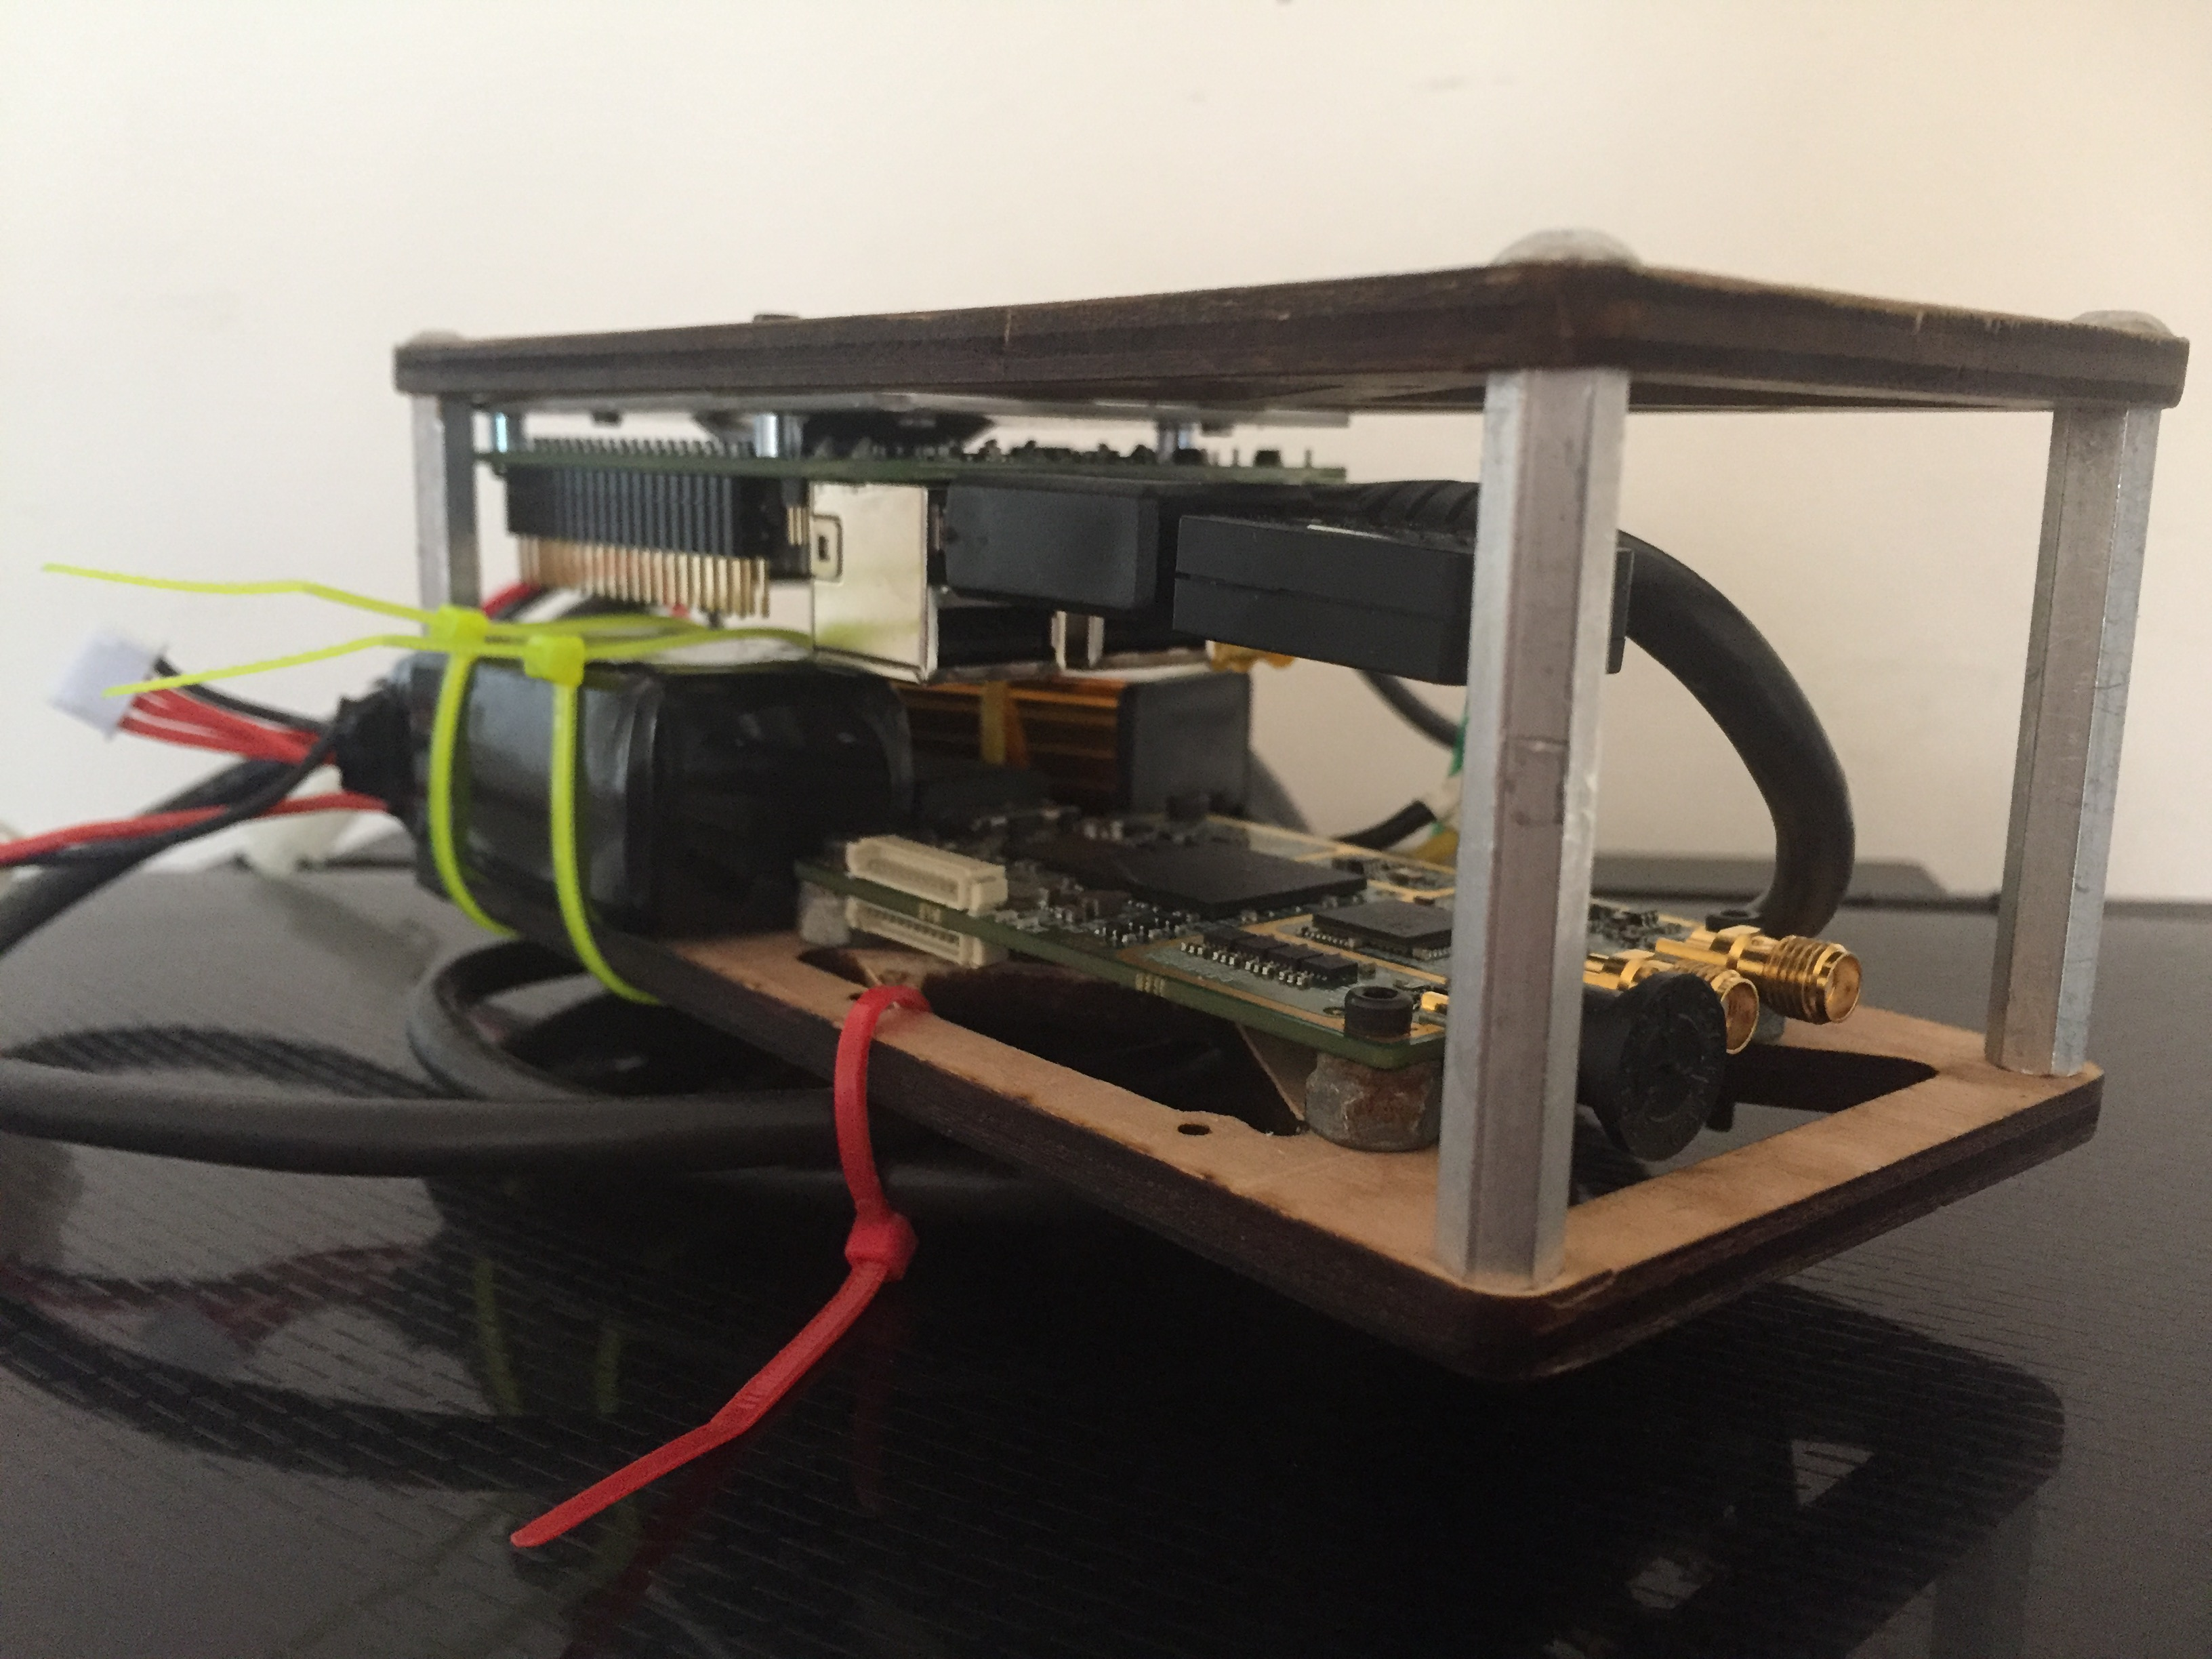
\includegraphics[width=0.70\textwidth]{img/box_usb_view.JPG}
	\caption{Angled side view of the encasing with the UP Board connected to the top panel with the GPS and USB cable to the B200-Mini. The golden transformer and the battery are positioned directly under the UP Board on the bottom panel. The B200-Mini is connected to the bottom panel and is the closes board to the camera.}
	\label{fig:box_usb_view}
\end{figure}\par
The GPS is connected to the UP Board using an micro USB to USB adapter. Integration and operation of the GPS proved to be a challenge. The GPSD library that was used to interface with the GPS had permission issues that caused the GPS data to not be read by a C++ program. After the permissions were set correctly, the MASDR program was able to correctly read the GPS data.\par

The magnetometer was to be connected to the UP Board using the I2C pins. Communication between the UP Board and the magnetometer was never established after multiple attempts. The UP Board would send a signal to the magnetometer, but never received a response. This could be due to a lack of a Linux driver or a faulty board. A Linux driver for the magnetometer wasn't provided by the manufacturer and the time line of the project made it unfeasible to write a driver by hand.\par

The B-200 mini was attached to the bottom panel of the casing. It communicated to the UP Board through a wired USB connection. The 900MHz and 2.4GHz antennas were connected to the SMA connectors on the mini. The 2.4GHz antenna required an adapter because the connector on the board was a smaller size than the one on the antenna. During testing, it was realized that the transmission from the board was not working. Upon further inspection it was noticed that a component had broken off the board. Another board was borrowed from a lab to verify that the original board was faulty. The transmission test ran successfully on the board from the lab. A working board and the broken board are shown in the Figure \ref{fig:working_mini} and Figure \ref{fig:broken_mini} respectively.
\begin{figure}[h]
	\centering
	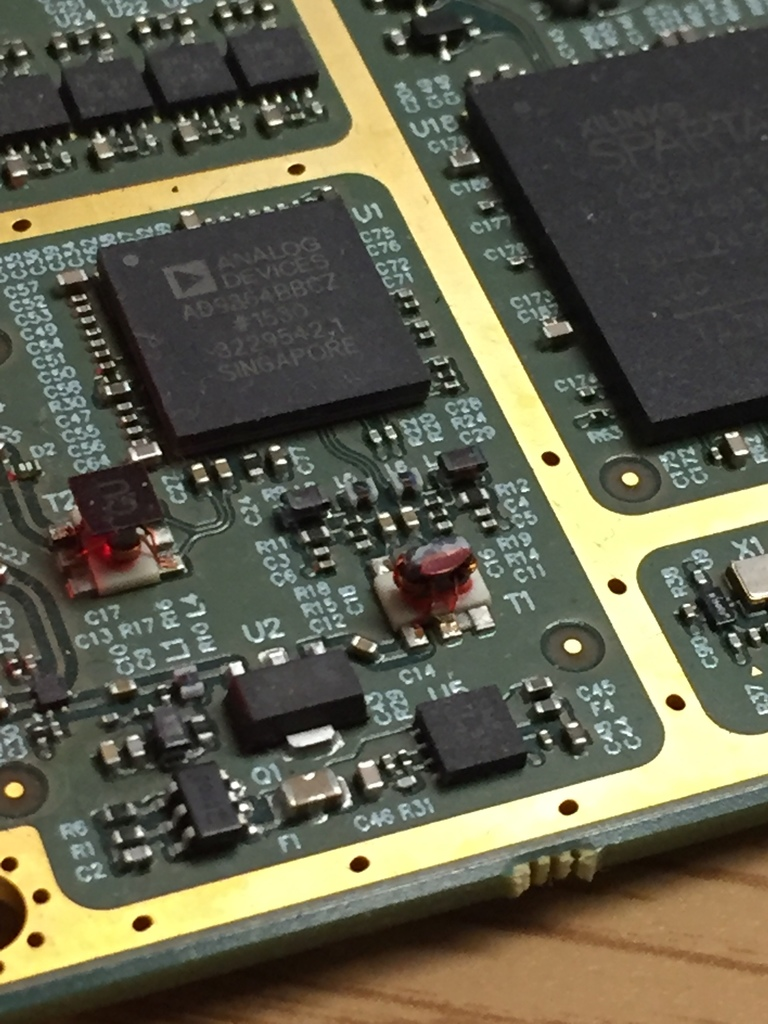
\includegraphics[width=0.70\textwidth]{img/working_mini.jpg}
	\caption{The functional B200-mini}
	\label{fig:working_mini}
\end{figure}
\begin{figure}[h]
	\centering
	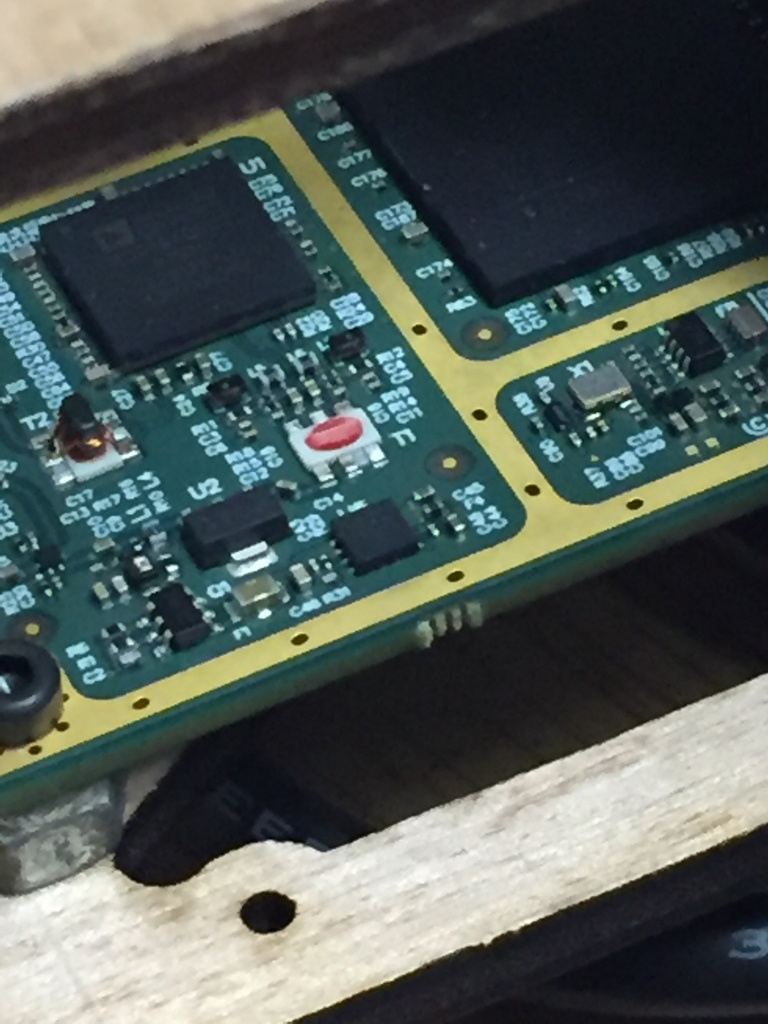
\includegraphics[width=0.70\textwidth]{img/broken_mini.jpg}
	\caption{The non-functional B200-mini}
	\label{fig:broken_mini}
\end{figure}
This component may have broken off during transport to and from meetings or because of vibrations during in flight testing. \par

The complete system mounted on the drone is shown in Figure \ref{fig:drone_and_box}.
\begin{figure}[h]
	\centering
	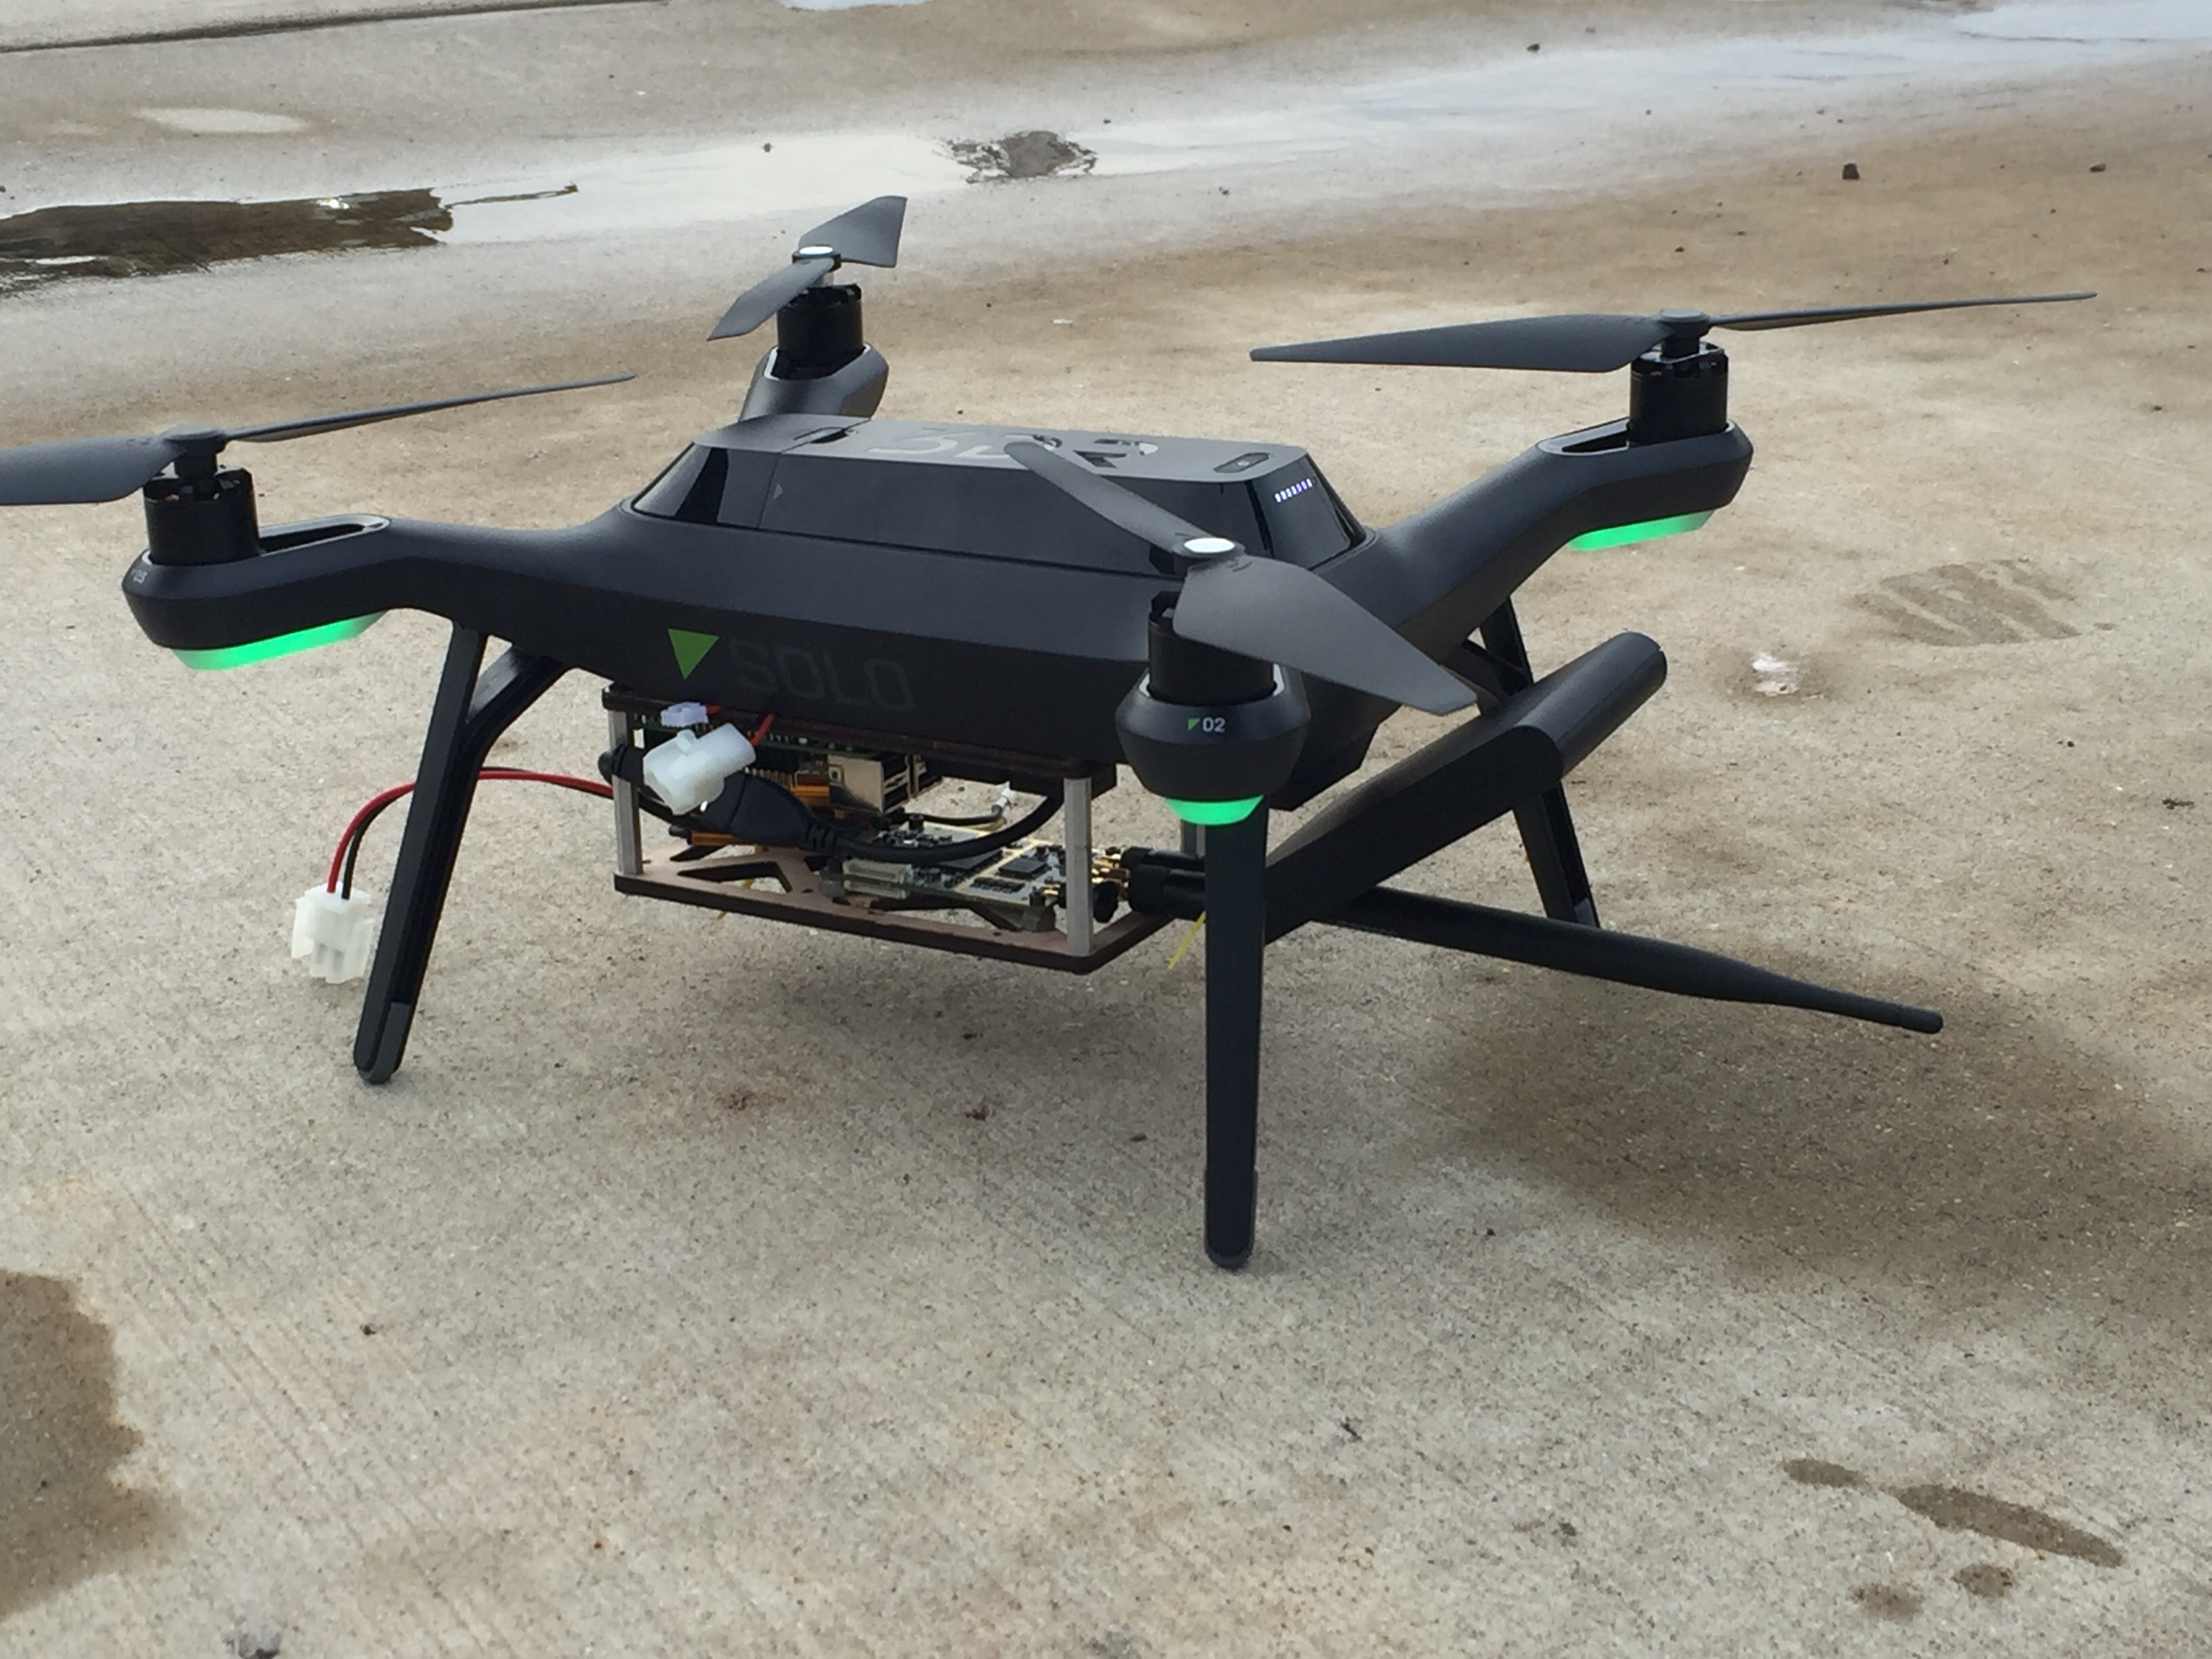
\includegraphics[width=0.70\textwidth]{img/drone_and_box.jpg}
	\caption{The complete system mounted on the drone. In flight testing was done with this setup.}
	\label{fig:drone_and_box}
\end{figure}
\par

\section{Code Framework}
Damn
\section{Drone Control}
To reduce interference when sensing signals, the WiFi cards on the controller and drone had to be replaced because the communication frequency and the sensing frequency matched. In order to replace these WiFi cards, research had to be done to determine the ath9k driver used which was compatible with a wide range of Atheros based cards. Despite the guarantee of compatibility, the first purchase of the R11e-5HnD MikroTik MiniPCI-E wireless card was unused due to the large heat sink that could not fit conveniently into both the controller and drone. Furthermore the connectors would also require adapters to connect to the antennas. This led to the second purchase of the SparkLAN WPEA-121N MiniPCI-E Half-Size wireless card, which required a bracket to be mounted. The replacement of the WiFi cards in the controller was done first for precaution and testing purposes. The replacement went smoothly, however the controller was still communicating at 2.4GHz. Upon checking the software, it detected that the WiFi card installed was capable of communicating at 5GHz. Therefore the controller's networking scheme was modified such that it would persistently communicate at a specific channel (5GHz). After these changes, SSHing into the controller was not possible. It was suspected that the antennas are incapable of transmitting at 5GHz. Limited with time and the scope of the project, it was not possible to obtain antennas to replace on the controller and drone. Due to this reason, the drone's WiFi card was not replaced, and both the controller and drone were factory reset to operate at 2.4GHz.

\section{Spectrum Sensing}
%RSS part of things.
%IQ_TO_FILE
In addition to calculating RSS values, a C++ program separate from the code framework
was written. This program, called iq\_to\_file, was created as a foundation with 
which to work with. It became the testbed for specific elements of MASDR, since it
was already capable of logging.The code for this section is in Appendix \ref{app:iq_to_file}. 
This program is built on the rx\_samples\_to\_file example that Ettus Research provides 
with the UHD. This program already had the desired base functionality, so it proved
to be a good starting point. The program was then stripped of unnecessary functionality,
including the command-line interface. \par
With the extraneous functionality removed, components of the MASDR framework were
added, in order to test them separately. The matched filter, RSS measurements, 
and GPS modules were added. This allowed for post-process localization. In order to 
save these values properly, they were packed into the complex type that was being
used to save IQ samples. In order to make it possible to pull these values out
in post-processing, they were given an unrealistic imaginary value. with each different 
module getting a different imaginarry value. The matched filter outputs got 
a flag of 1000. GPS X, Y and Z coordinates were given flags of 2000, 3000, and 4000,
respectively. RSS values got a flag of 5000. These values were written with each 
buffer of samples received. This makes it easier to align results when processing.\par
%MATLAB
Once a data file was recorded, it was processed using a MATLAB script. This script 
is in Appendix \ref{app:matlab_proc}. This script reads in the .dat file produced 
by iq\_to\_file, as floats. It then separates the data into in-phase and quadrature
components. Then, after pre-allocating buffers, the script pulls out the non-IQ 
samples. The matched filter values and the RSS measurements are then plotted. The
script used to plot the received signal, but with longer record times, this
becomse impractical or impossible.

\section{Spectrum Localization}
%GPS in general
%GPS from drone
In order to use the data gathered in the test conducted on December 11, 2016, GPS 
data was pulled from the drone. This was done using a command-line interface that 
3DR provided online \cite{3dr_devguide}. Unlike the other logs that were pulled using this method,
the GPS information was loggeed in a Dataflash log. This format saves the information
in MAVlink packets, making it easier to transmit to a base station but harder
to post-process. To deal with this, the Ardupilot Mission Planner software was 
installed \ref{ard_mplanner}. This software is capable of taking the dataflash logs
generated by the 3DR Solo and converting them into a format that's easier to
process. Using this software, the logs for the flight on December 11, 2016 were 
converted to MATLAB data files. The relevant GPS information was then pulled from
the larger data set.
%Probably put script here
%KF Simulation


\section{Transmit To Ground}
\section{Summary}
